\documentclass[11pt]{article}
\usepackage{a4,caption,listings,graphicx,enumerate,amsmath,amssymb,mathtools,lipsum,graphicx,microtype,float,xcolor, multicol}
\usepackage[a4paper,margin=1in,footskip=0.25in]{geometry}
\usepackage[rightcaption]{sidecap}

\title{\line(1,0){450} \\ \Huge\textbf{Insights through asymptotics:}\\
 \LARGE Benchmarking and analysis of climate effects on flood models}
\author{Henry Writer }
\date{\today}

\usepackage{titlesec}
\renewcommand{\thesection}{\Roman{section}}

\titleformat{\section}[block]{\LARGE\bfseries\filcenter\titlerule\vspace{2mm}}{\thesection}{1em}{}

\titleformat{\subsection}[block]{\Large\bfseries\filcenter}{}{1em}{}

\begin{document}

\maketitle

\section{Background}

There is currently unmistakable evidence that the climate of the planet is changing. We currently do not understand what the potential outcomes of these changes may be. One route we have to understand these changes takes the form of models these models then can be used to help us predict the future impact of climate change.

In the United Kingdom one of the largest potential effects of climate change we will take the form of river flooding. The government cost the 2015/16 floods at 1.6 billion pounds. This number does not take into account the human toll of this event. Additionally, it appears that the number and severity of flooding is increasing. 


This has motivated the hydrological community in increasing the understanding of river flooding. This has been done by developing a 'zoo' of potential flooding models. However, there are two problems regarding this large group of models. One since there is so many it is hard to separate them REF. 
Secondly we believe there is still information which is not being extracted from these models that can help us predict how flooding will change. We believe that we can solve both of these problems by examining models using asymptotic analysis.

\subsection{How do we model river flooding}
There are currently three main approaches to flooding model. We have statistical models this realy on using statistical method to fit models to data and use statistical models to make inferences about the future. 
We have conceptual models, these realy in creating a set of states from which water can move between this is best represented by a FIGURE. 
Finaly we have physical models these take a continuime mechanics approch and set up a set of conservation laws and use these to drive a set PDE sytems that can be used to mdoel the flooding event.



\subsection{Conceptual models}

 As briefly mentioned in the previous section conceptual models attempt to capture a complex system such as river flooding and simplify it down to a set of possible states/locations the variable of interest may reside in. Travel between these states is then governed by a simple mathematical expression.
 
 \begin{minipage}{0.5\textwidth}
    \begin{figure}[H]
        \centering
        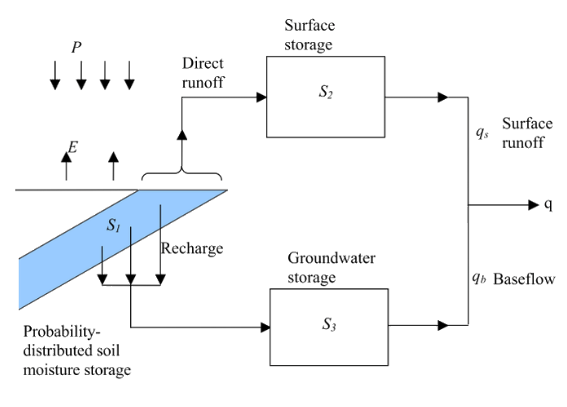
\includegraphics[width=1\textwidth]{Figs/Concept.png}
        \caption{Example of a Conceptual model}
        \label{fig:conceptual}
    \end{figure}
\end{minipage}
\begin{minipage}{0.4\textwidth}
    Figure \ref{fig:conceptual} gives a diagrammatic example of a conceptual model this model show how rain water might flow through a catchment area. It shows rain entering the system precipitation and how the path it might take, either evaporating immediately, or by flowing into surface or groundwater storage, before being eventually discharged.
\end{minipage}

\vspace{1cm}
\begin{minipage}{0.3\textwidth}
    We can see that conceptual modelling allow us to easily build a model that in can incorporate many aspects of a system. However, with such in designing these models means that there is a `zoo' of similar models from which we could use to model a potential river catchment area. This issue of benchmarking these models to determine which one is mots suitable for a given situation are discussed in REFRENCE, 

    Figure \ref{fig:eaBench}  graphically demonstrates the challenge posed in differentiating flooding models. This is one of the major motivations of the proposed assytopic benchmarking process.
\end{minipage}
\begin{minipage}{0.6\textwidth}
    \begin{figure}[H]
        \centering
        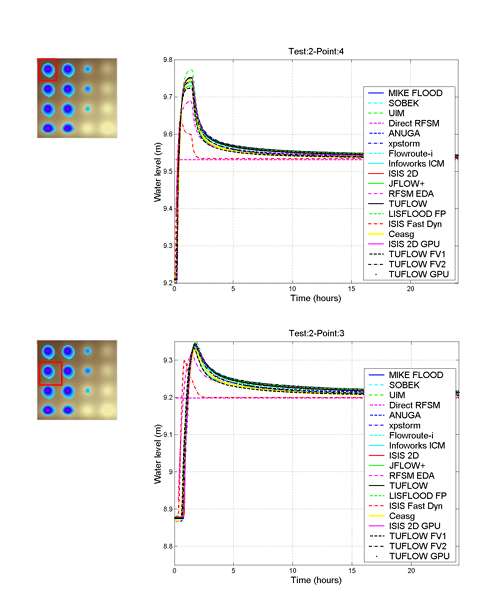
\includegraphics[width=0.75\textwidth]{Figs/EA_bench.png}
        \caption{Ahhhhhhhhhhhhhhhhhhhhhh}
        \label{fig:eaBench}
    \end{figure}
\end{minipage}







\subsection{How do we currently interpret the output of flooding models}


Another motivation to creating a methodology to derive scaling laws from conceptual models is in the predication of future flooding events. The method currently used to give predictions of future flooding evolves taking a handful of different data sets that model a potential climate under a variety of possible climate situations. These data sets are then feed in to a conceptual model then these outcomes are used to draw inferences about future floods.
This process can be visualised in the flow diagram in Figure \ref{fig:flow}.

\begin{figure}[H]%this figure will be at the left
    \centering
    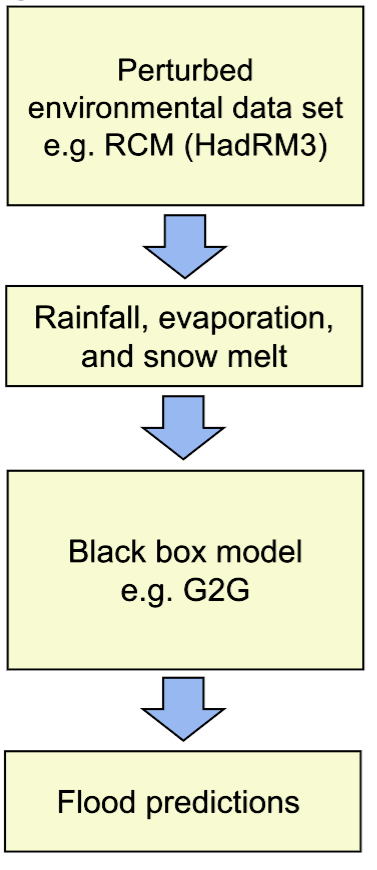
\includegraphics[width=0.2\textwidth]{Figs/flow.png}
    \caption{I hate the warp enviroment}
    \label{fig:flow}
\end{figure}

The paper by PEOPLE is a good reference for how this process is carried out in practice. Figure \ref{fig:concept_in} shows the diffreent rainfa;; data entered in to the model, and Figure\ref{fig:concept_out} show the output form there model. They then use the output form these models to make simple predictions about the effect of climate change.

We think that our assintpic benchmarking process that we can do better by deriving psychical scaling laws that will can give additional insight in to flooding.

\begin{figure}[H]%this figure will be at the left
    \centering
    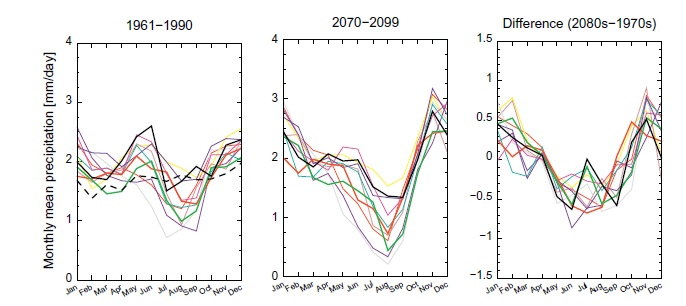
\includegraphics[width=0.5\textwidth]{Figs/concept_in.jpg}
    \caption{Mmmmmmmmmmmmmmmmmmmmmmmmmmmmmm}
    \label{fig:concept_in}
\end{figure}

\begin{figure}[H]%this figure will be at the left
    \centering
    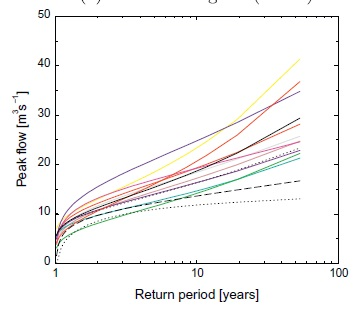
\includegraphics[width=0.5\textwidth]{Figs/concept_out.jpg}
    \caption{Nooooooooooooooooooooooooooooooooooo}
    \label{fig:concept_out}
\end{figure}




\subsection{Reduced PDE model}


\section{Problem formulation and method}

\subsection{A new approach to benchmarking}


\subsection{Extending the model with periodic forcing}

\section{Objectives and strategy}

The work outlined above is designed to be undertaken as PhD project. A potential student undertaken this project would require a strong background in fluid mechanics, asymptotic analysis and, would require a passion for environmental mathematics. 
Additionally, it would be beneficial if a potential student had some experience with time series analysis, and numerical PDEs.

\subsection{Objectives}
Below is a list of initial targets which shall form the core of the project.

\begin{enumerate}
    \item \textbf{Numerical derive scaling laws,} from conceptual models. This would require conducting a literature review to ascertain influential models that our benchmarking method could be applied to.
    \item \textbf{Analytically derive scaling laws,} this shall be accomplished by using numerical laws derived to inform a discretion of the conceptual models. To conduct this integration we shall use asymptotic analysis.
    \item \textbf{Apply periodic rainfall to the reduced PDE model}. To this end we will need to conduct a time series analysis of rainfall data. This shall be used to find appropriate time scales to inform the analysis of the reduced PDE model.
\end{enumerate}

\subsection{Potential future objectives}

There are a number of directions this project may be extended dependent upon the interests of the student. A couple of potential avenues of extension are outlined below to show the scope of where this project.

The reduced PDE model has a number of other extension which can be explored. One approach would be to use the astytotic method of homisation, this would allow us to explore how a more complex soil structure will effect flooding events. Another approach we could use to examine the water flow in soil would be to replace the equation which governs the flow through the soil with a conduit equation this would allow us to explore channelling behaviour in the soil.

We could also take a dynamical systems approach to analys ing the reduced PDE model. For example it very natural to assume that there is two possible states in which a catchment area could be in, a staturated state this would be equivalent to a wetland, and a dry/draught state. We then assume that as the land dry out it becomes less pouress so more watter flows direclty overland. We can then explore how much rainfall would have to change to transition between these states.

Another promesing avenuea we could explore would be attemtping to match the conceptual models with the reduced PDE model. This would be of great intrested as the different methoglgies for building flooding models are metphoricaly existe on seprated islands. By matching the PDE modle to a conceptual model we hope to be able to connect these modles to gether.

These free possible reasrech direction are not ment to be taken as a demenstartion of the scope of this projetc and it postential.



\section{Impact}
Like all research proposal we believe that we are carrying out novel and interesting mathematics. Additionally due to the subject of this research on climate change and namely river flooding which is one of a major extensional threat to the United Kingdom and the wider world. Any additional understanding of flooding mechanics and additional predictions will prove to be extremely valuable.
\subsection{Mathematical impact}
To emphasise the mathematical impact of this project here is a non-exhaustive list of the novel mathematics. 
\begin{enumerate}
    \item Applying assytopic methods to derive scaling laws for climate models is a potential new application for these methods.
    \item A deep analytical analysis of conceptual modelling methods we will help to give understanding of how these commonly used techniques will behaviour.
    \item The application of a multiple time scales analysis to the reduced PDE models is very likely to generate new and interesting problems which will need to be solved.
\end{enumerate}

\subsection{Industrial impact}
As this problem has been brought forward by the Environments Agency and ??????????? there is a clear interest in this type of work. But more concretely there is a very large motivation from practising hydrologists for a rigours analysis of the conceptual models that for the foundation of there practice. Additionally, we believe that the scaling laws that will be derived during this process may help to inform how we manage the risks of river flooding.

Finally, the second strand of this project in extending the PDE model to incorporate periodic forcing we will allow us to help examine seasonl rainfall and examine/predict chages in potential flooding over the timescale of climate change. This type of analysis is challenging for industry to carry out and is prime territory for a PhD project.




\section{References}

\end{document}